\begin{figure}[htbp]\centering
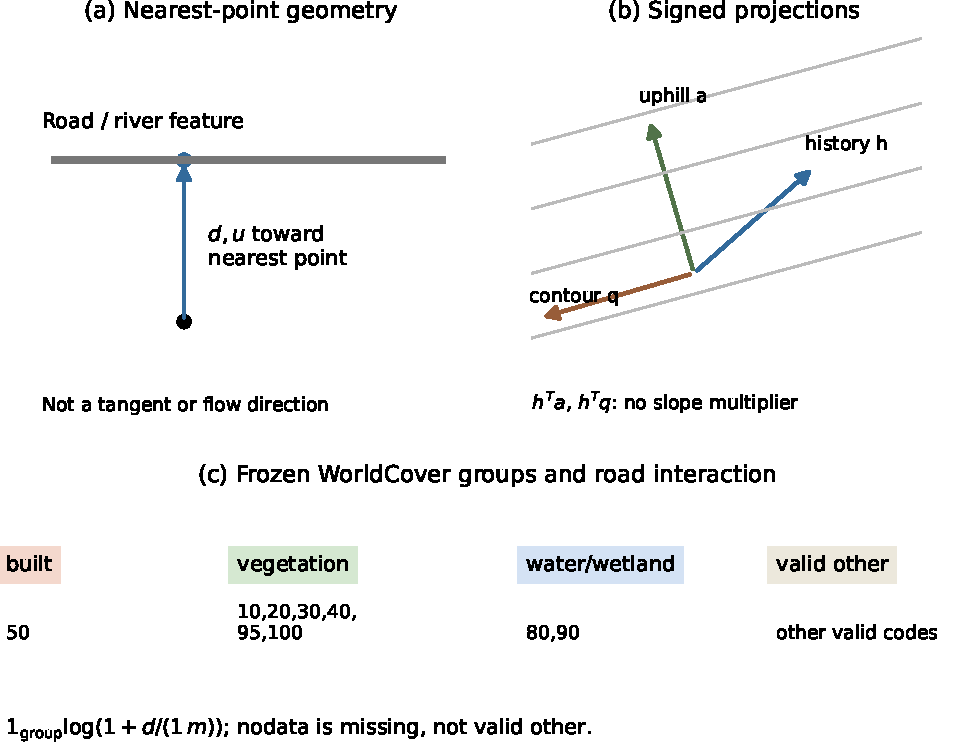
\includegraphics[width=\linewidth]{../figures/reader-v2/geometry.pdf}
\caption{Input geometry (three schematic panels, no measured effect).
Distance and direction point toward the nearest feature; signed uphill and
contour projections do not include a slope multiplier. Slope magnitude is
a separate input, not depicted here. The frozen WorldCover groups are built
(50), vegetation (10/20/30/40/95/100), water/wetland (80/90), and other valid
codes. Invalid or nodata values are missing, not ``other''.}
\label{fig:input-geometry}\end{figure}

\begin{figure}[htbp]\centering
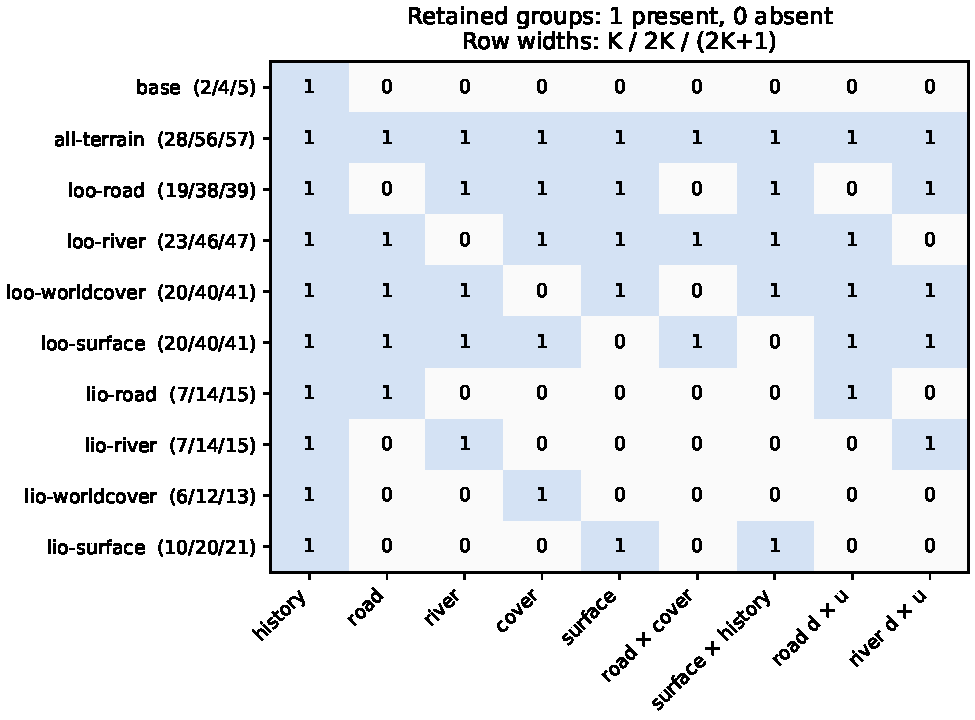
\includegraphics[width=\linewidth]{../figures/reader-v2/design.pdf}
\caption{Ten configurations by nine group/dependency columns: 90 design
states, not measurements. $K$ counts numerical features, $2K$ includes their
masks and $2K+1$ includes the intercept; these are not fitted rank or degrees
of freedom. Every row retains history. Road--cover requires both parent
groups and surface--history remains in LIO-surface.}
\label{fig:input-design}\end{figure}
The overall comparison is all-terrain minus base. Leave-one-out (LOO)
compares all-terrain with all-minus-group; leave-one-in (LIO) compares
history-plus-group with base. A negative candidate-minus-control score
favours the candidate. Describing a removal loss as factor benefit reverses
the sign and maps an interval $[l,u]$ to $[-u,-l]$. The dependent columns
in Figure~\ref{fig:input-design} explain why removing one group can remove
several numerical features. This design description remains useful even
when required failures prevent the registered terrain inference.
\FloatBarrier
